\chapter[Resultados]{Resultados}
\label{ch:resultados}
% TER EM MENTE:
% Refere-se à apresentação em ordem lógica dos resultados obtidos, sem interpretação pessoal do autor. Devem ser apresentados de forma objetiva, precisa e lógica, utilizando tabelas, gráficos, figuras etc.

% APENAS PARA ILUSTRAR O TIPO DE PLOTS QUE PRETENDO COLOCAR
% CONSIGO REFAZER QUALQUER PLOT FACILMENTE
% TENHO INFORMAÇÃO/DADOS PARA GERAR DIVERSOS PLOTS E TESTES OFFLINE

% OBJETIVO:
% 1) MOSTRAR O RESULTADO DA CALIBRAÇÃO (CURVA ESTIMADA X DADOS BRUTOS)
% 2) MOSTRAR O RESULTADO DA FILTRAGEM; COMPARAR COM FILTOS SIMPLES (POSSO APLICAR OS FILTROS OFFLINE NOS DADOS COLETADOS)
% 3) MOSTRAR O RESULTADO DO CONTROLE, PRINCIPALMENTE COM O INTUITO DE DIMINUIR AS ASSIMETRIAS DOS MOTORES

% MOSTRAR:
% RESPOSTAS PARA DIFERENTES CONFIGURAÇÕES DE MOTOR-SENTIDO E COM DIFERENTES REFERENCIAS/SINAIS DE CONTROLE PARA:
% CURVA ESTIMADA X SEM FILTRO X COM FILTRO
% \section{Resultados da calibração}

% Please add the following required packages to your document preamble:
% \usepackage{graphicx}
\begin{table}[H]
\centering
\resizebox{\textwidth}{!}{%
\begin{tabular}{c|cc|cc|cc|cc}
\multicolumn{1}{r|}{\textbf{}} &
  \multicolumn{2}{c|}{\textbf{$K_m$ {[}rad/s{]}}} &
  \multicolumn{2}{c}{\textbf{$\tau_m$ {[}s{]}}} &
  \multicolumn{2}{c|}{\textbf{$K_p$ {[}$1/(rad/s)${]}}} \\
\textbf{Experimento} &
  \textbf{\begin{tabular}[c]{@{}c@{}}Motor\\ Esquerdo\end{tabular}} &
  \textbf{\begin{tabular}[c]{@{}c@{}}Motor\\ Direito\end{tabular}} &
  \textbf{\begin{tabular}[c]{@{}c@{}}Motor\\ Esquerdo\end{tabular}} &
  \textbf{\begin{tabular}[c]{@{}c@{}}Motor\\ Direito\end{tabular}} &
  \textbf{\begin{tabular}[c]{@{}c@{}}Motor\\ Esquerdo\end{tabular}} &
  \textbf{\begin{tabular}[c]{@{}c@{}}Motor\\ Direito\end{tabular}} \\ \hline
\textbf{1} &
  3236.80 &
  3047.72 &
  7.62e-02 &
  6.57e-02 &
  1.37e-04 &
  1.24e-04 \\
\textbf{2} &
  4446.69 &
  4514.56 &
  5.71e-02 &
  5.40e-02 &
  3.01e-05 &
  3.23e-05 \\
\textbf{3} &
  4335.81 &
  4394.23 &
  5.48e-02 &
  5.30e-02 &
  1.54e-05 &
  2.11e-05 \\
\textbf{4} &
  3345.83 &
  3644.55 &
  4.43e-02 &
  5.90e-02 &
  5.55e-05 &
  3.80e-05
\end{tabular}%
}
\caption{Resultado da calibração para os diferentes experimentos.}
\label{tab:resumo_calibracao}
\end{table}


\begin{figure}[H]
    % \centering
    \begin{subfigure}{.5\textwidth}
    \centering
    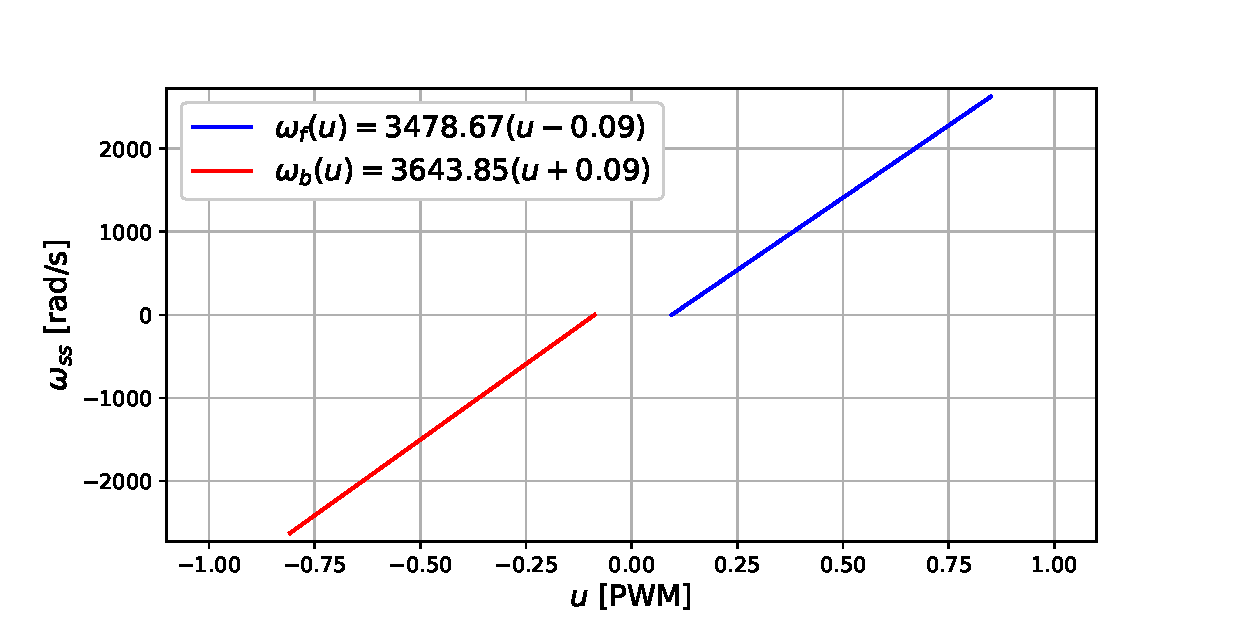
\includegraphics[width=\textwidth]{figuras/resultados/exp01/curva_feedforward_esquerdo100.eps}
    \caption{Curva $u(\omega)$ para o motor esquerdo.}
    \end{subfigure}
    \hfill
    \begin{subfigure}{.5\textwidth}
    \centering
    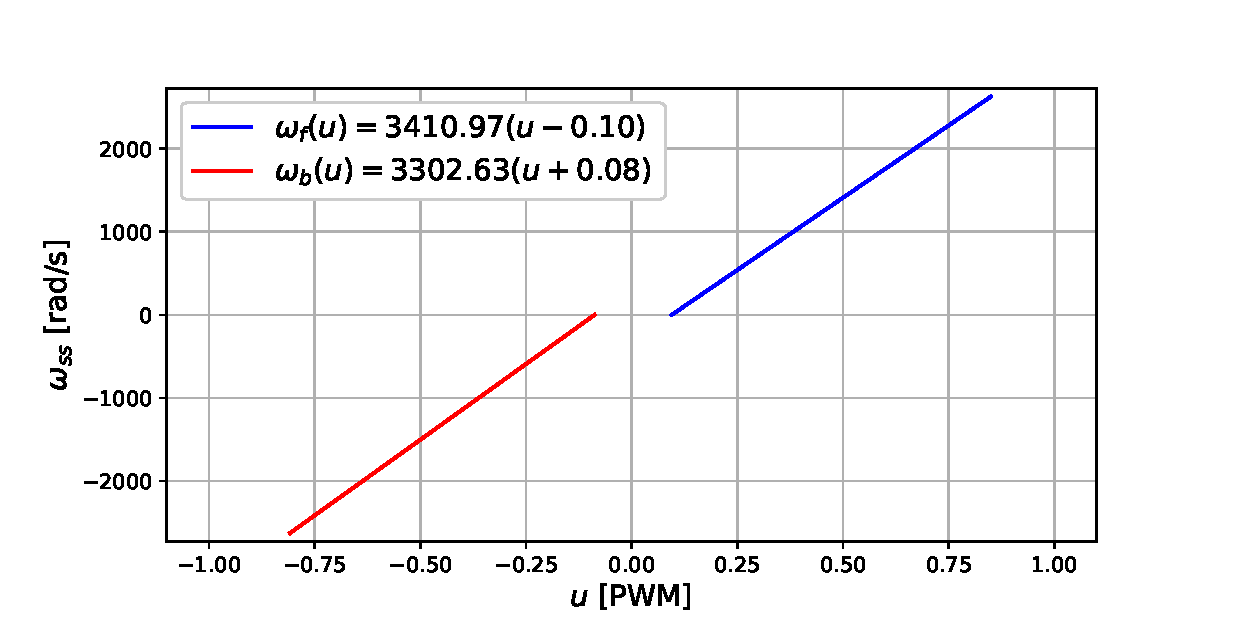
\includegraphics[width=\textwidth]{figuras/resultados/exp01/curva_feedforward_direito100.eps}
    \caption{Curva $u(\omega)$ para o motor direito.}
    \end{subfigure}
    \begin{subfigure}{.5\textwidth}
    \centering
    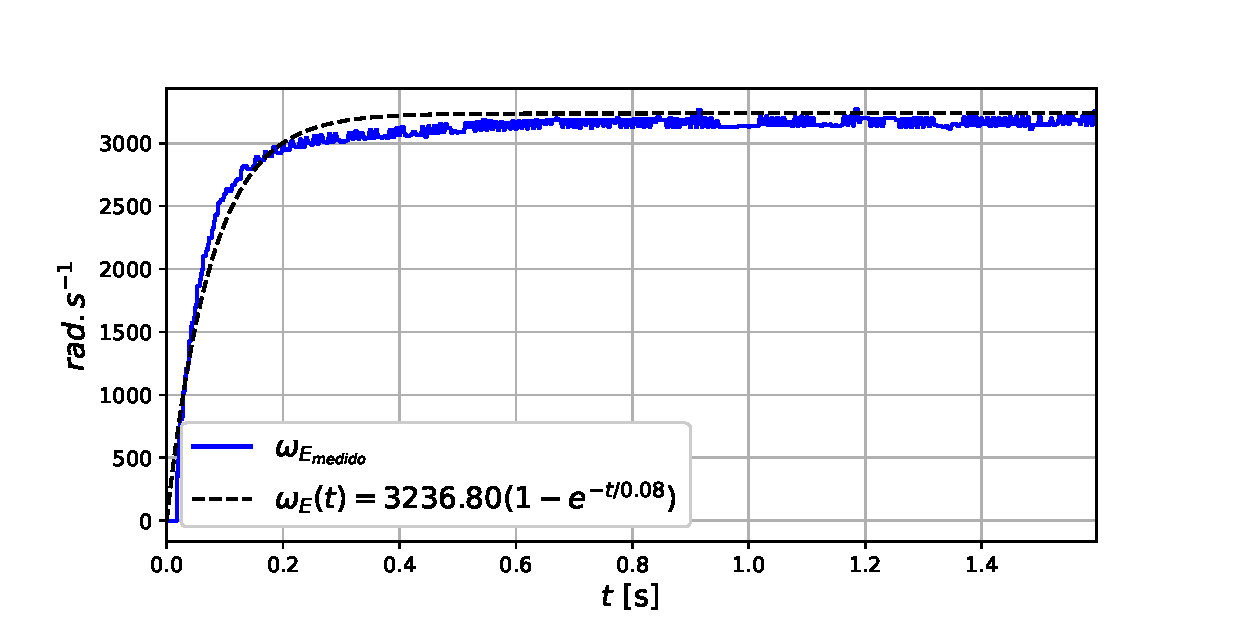
\includegraphics[width=\textwidth]{figuras/resultados/exp01/regressao_vs_medido_esquerdo100.eps}
    \caption{Curva $\omega(t)$ ideal, com os parâmetros da identificação vs velocidades medidas. Motor Esquerdo.}
    \end{subfigure}
    \hfill
    \begin{subfigure}{.5\textwidth}
    \centering
    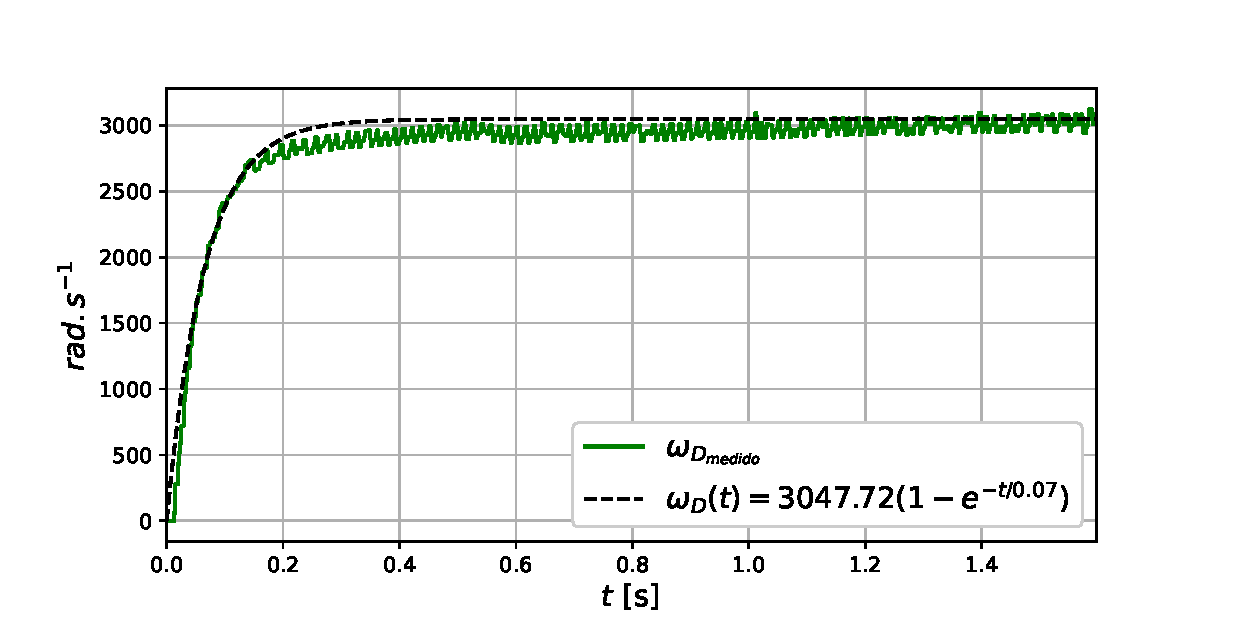
\includegraphics[width=\textwidth]{figuras/resultados/exp01/regressao_vs_medido_direito100.eps}
    \caption{Curva $\omega(t)$ ideal, com os parâmetros da identificação vs velocidades medidas. Motor Direito.}
    \end{subfigure}
    \hfill
    \begin{subfigure}{.5\textwidth}
    \centering
    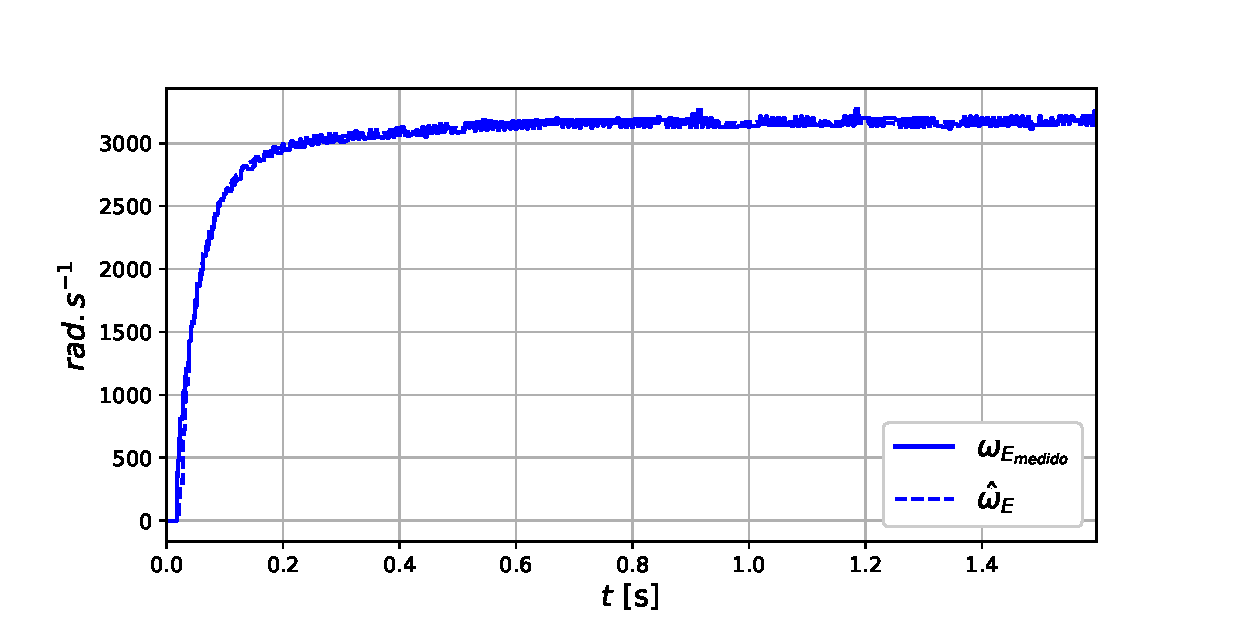
\includegraphics[width=\textwidth]{figuras/resultados/exp01/filtro_vs_sem_filtro_esquerdo100.eps}
    \caption{Comparação entre a velocidade estimativa $\hat{\omega}$ e a velocidade $\omega$ medida. Motor Esquerdo.}
    \end{subfigure}
    \hfill
    \begin{subfigure}{.5\textwidth}
    \centering
    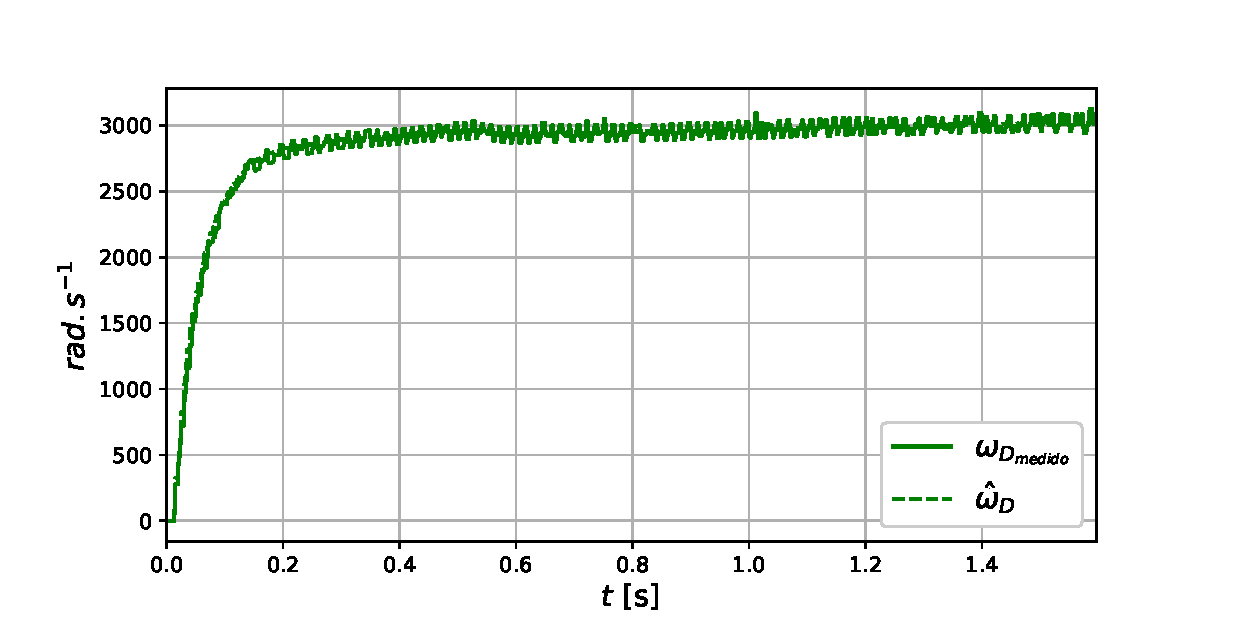
\includegraphics[width=\textwidth]{figuras/resultados/exp01/filtro_vs_sem_filtro_direito100.eps}
    \caption{Comparação entre a velocidade estimativa $\hat{\omega}$ e a velocidade $\omega$ medida. Motor Direito.}
    \end{subfigure}
    \hfill
    \begin{subfigure}{.5\textwidth}
    \centering
    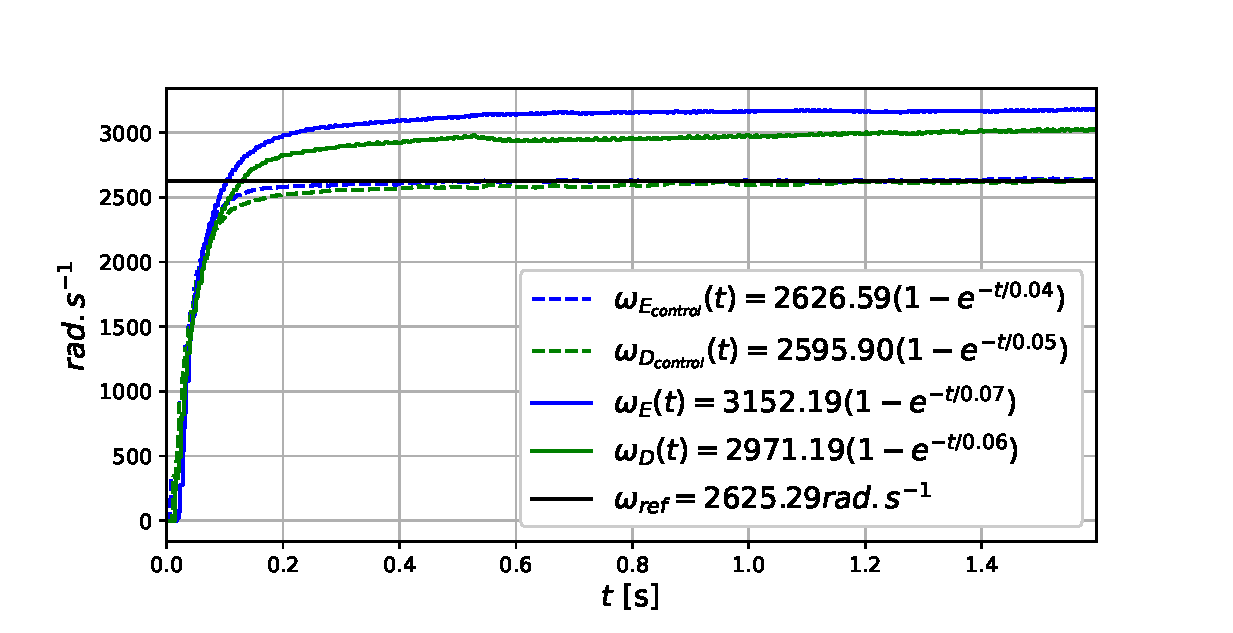
\includegraphics[width=\textwidth]{figuras/resultados/exp01/controlador_vs_sem_controlador100.eps}
    \caption{Comparação entre o sistema com controlador vs sem controlador.}
    \end{subfigure}
    \hfill
    \begin{subfigure}{.5\textwidth}
    \centering
    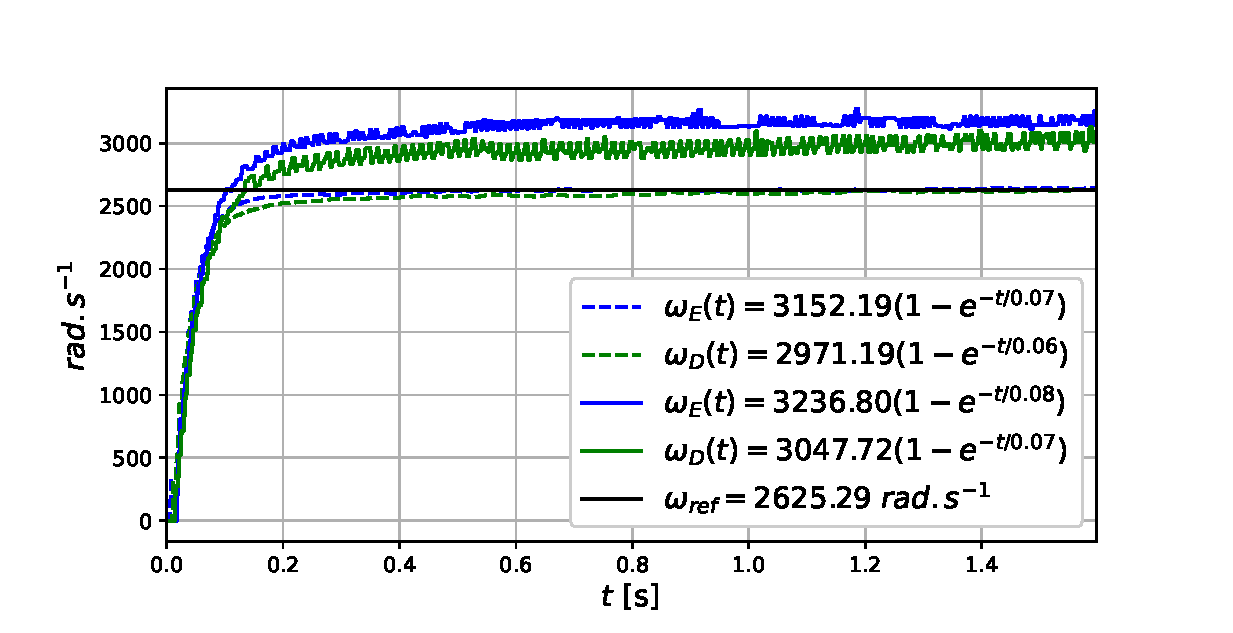
\includegraphics[width=\textwidth]{figuras/resultados/exp01/antes_vs_depois100.eps}
    \caption{Resposta sem observador e sem controle vs com controlador e observador.}
    \end{subfigure}
    
    \caption{Experimento 1. \emph{Sinal de controle e Referência igual a 1.0.}}
    \label{fig:exp01_100}
\end{figure}


\begin{figure}[H]
    % \centering
    \begin{subfigure}{.5\textwidth}
    \centering
    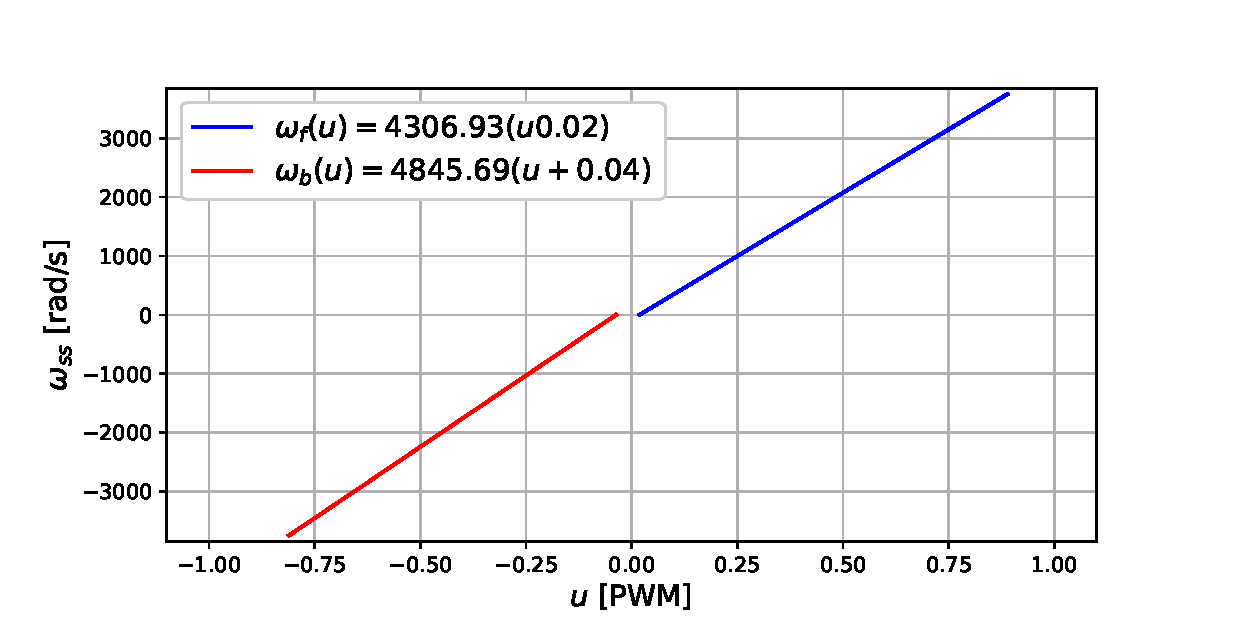
\includegraphics[width=\textwidth]{figuras/resultados/exp02/curva_feedforward_esquerdo100.eps}
    \caption{Curva $u(\omega)$ para o motor esquerdo.}
    \end{subfigure}
    \hfill
    \begin{subfigure}{.5\textwidth}
    \centering
    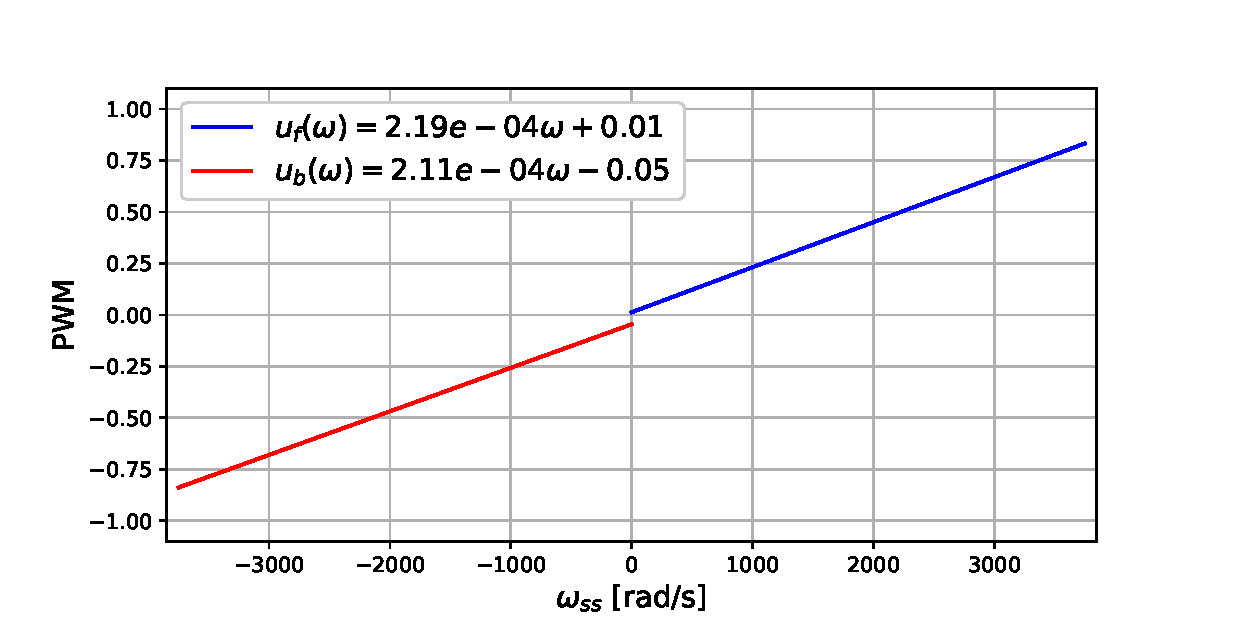
\includegraphics[width=\textwidth]{figuras/resultados/exp02/curva_feedforward_direito100.eps}
    \caption{Curva $u(\omega)$ para o motor direito.}
    \end{subfigure}
    \begin{subfigure}{.5\textwidth}
    \centering
    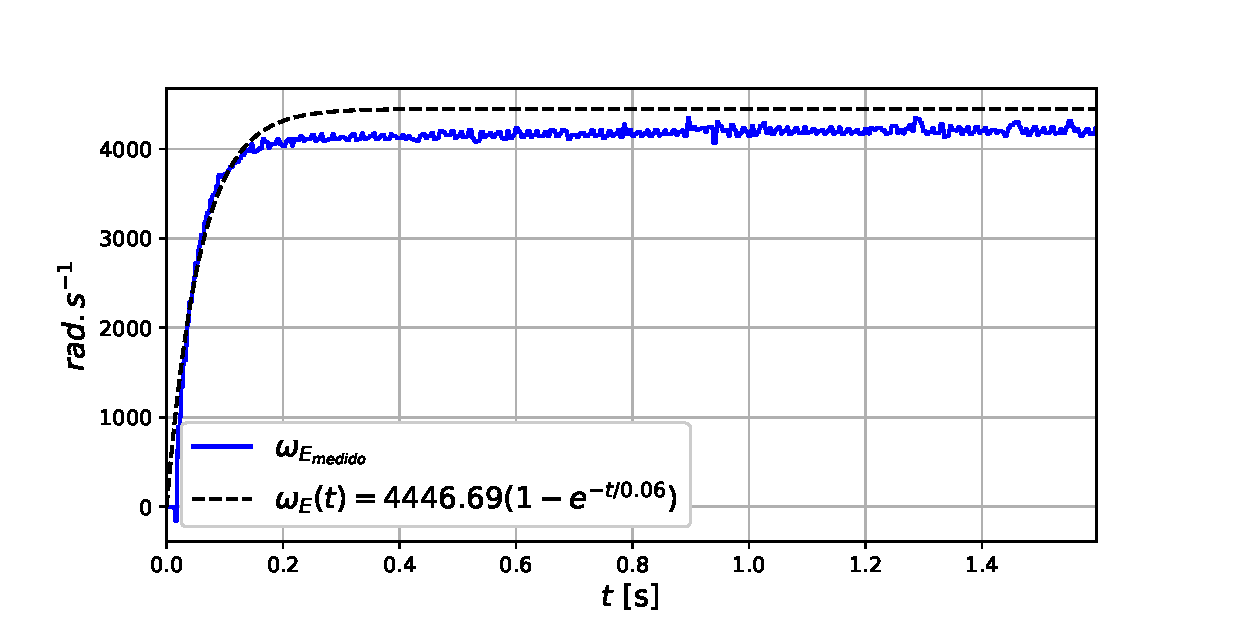
\includegraphics[width=\textwidth]{figuras/resultados/exp02/regressao_vs_medido_esquerdo100.eps}
    \caption{Curva $\omega(t)$ ideal, com os parâmetros da identificação vs velocidades medidas. Motor Esquerdo.}
    \end{subfigure}
    \hfill
    \begin{subfigure}{.5\textwidth}
    \centering
    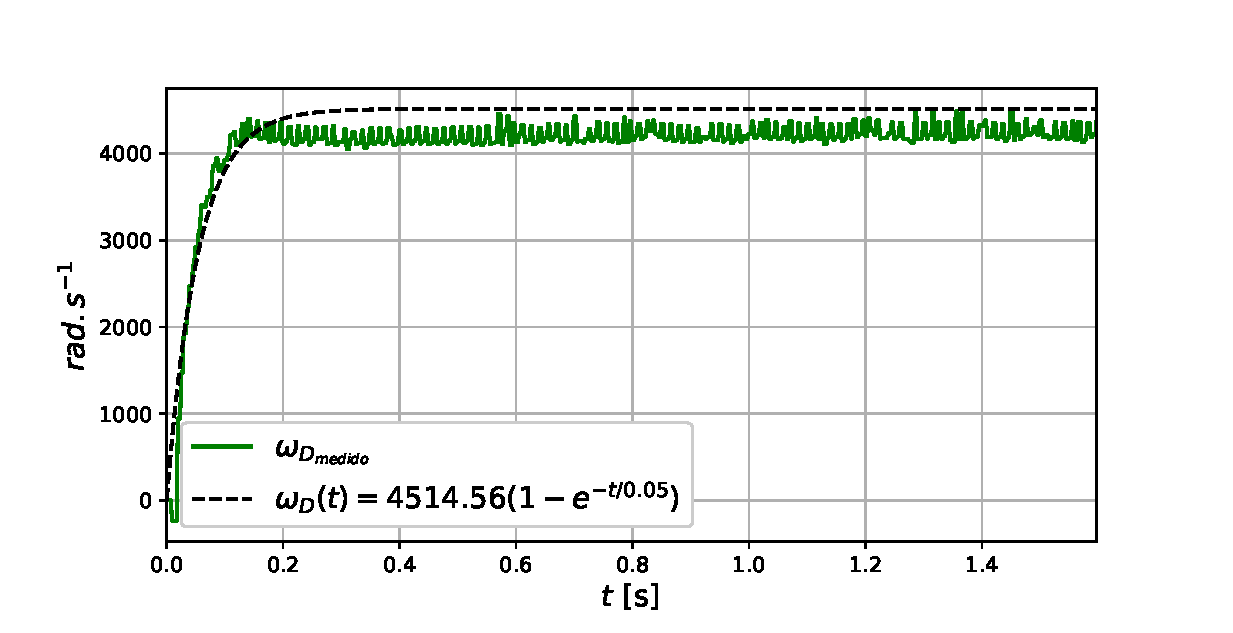
\includegraphics[width=\textwidth]{figuras/resultados/exp02/regressao_vs_medido_direito100.eps}
    \caption{Curva $\omega(t)$ ideal, com os parâmetros da identificação vs velocidades medidas. Motor Direito.}
    \end{subfigure}
    \hfill
    \begin{subfigure}{.5\textwidth}
    \centering
    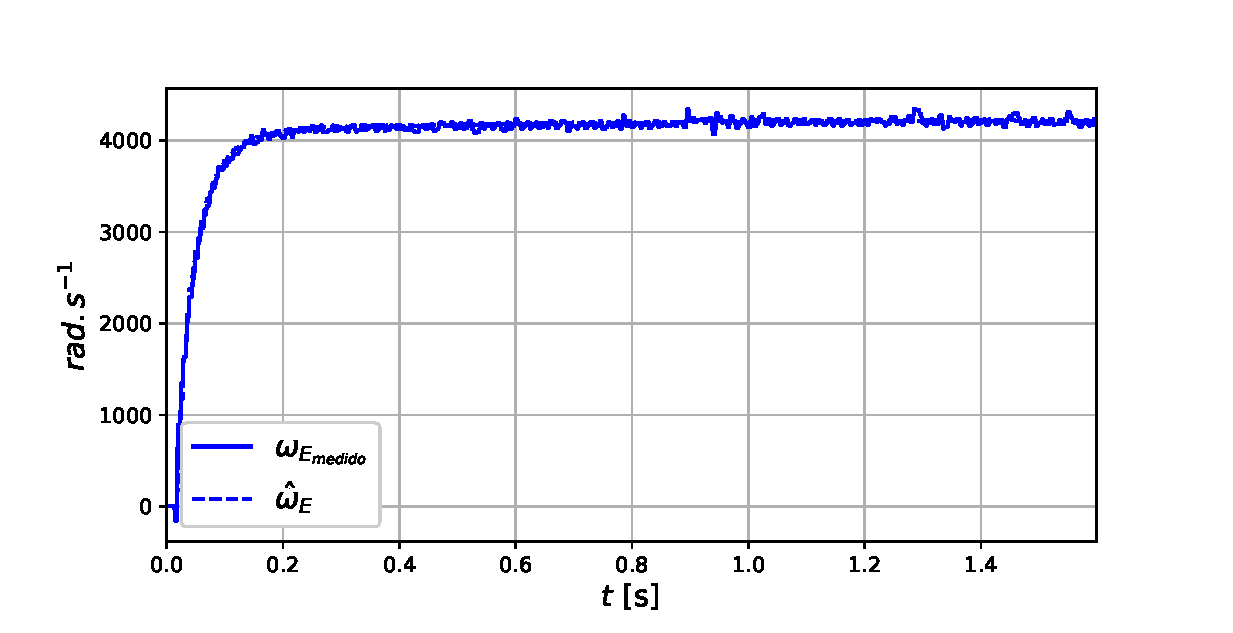
\includegraphics[width=\textwidth]{figuras/resultados/exp02/filtro_vs_sem_filtro_esquerdo100.eps}
    \caption{Comparação entre a velocidade estimativa $\hat{\omega}$ e a velocidade $\omega$ medida. Motor Esquerdo.}
    \end{subfigure}
    \hfill
    \begin{subfigure}{.5\textwidth}
    \centering
    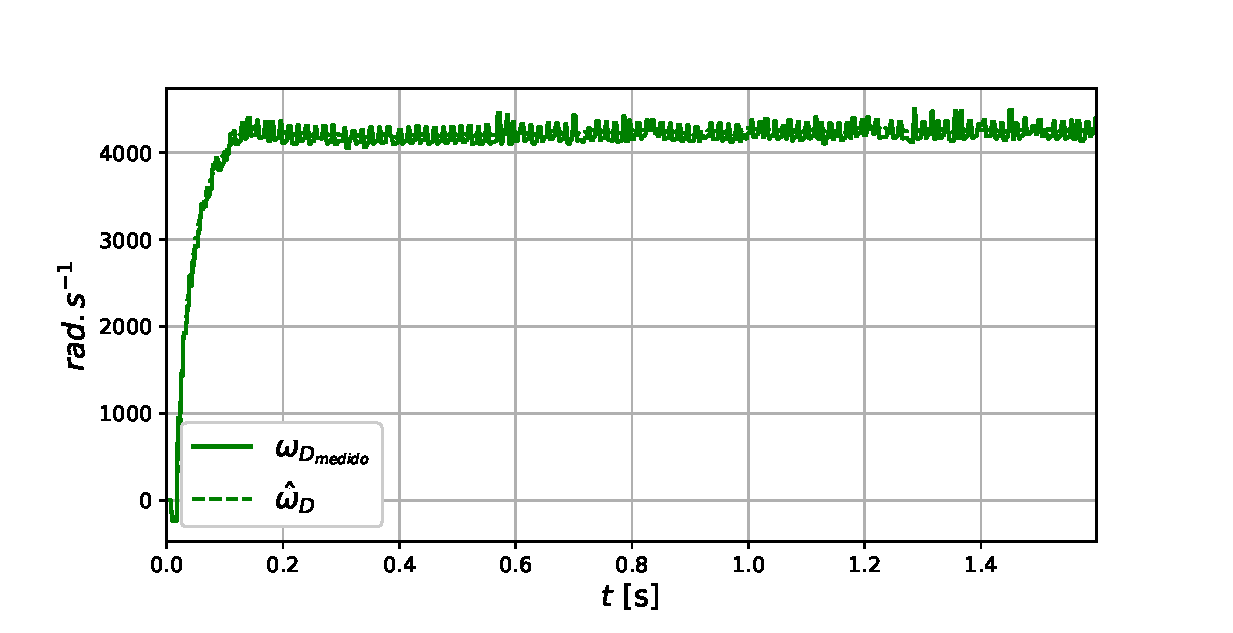
\includegraphics[width=\textwidth]{figuras/resultados/exp02/filtro_vs_sem_filtro_direito100.eps}
    \caption{Comparação entre a velocidade estimativa $\hat{\omega}$ e a velocidade $\omega$ medida. Motor Direito.}
    \end{subfigure}
    \hfill
    \begin{subfigure}{.5\textwidth}
    \centering
    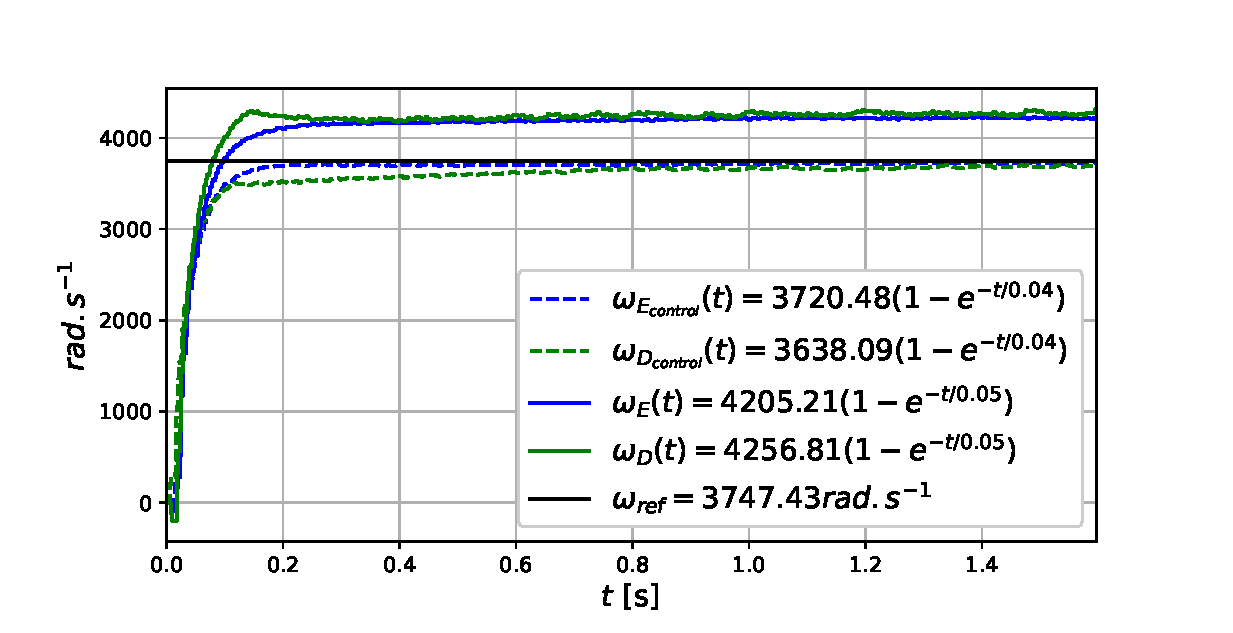
\includegraphics[width=\textwidth]{figuras/resultados/exp02/controlador_vs_sem_controlador100.eps}
    \caption{Comparação entre o sistema com controlador vs sem controlador.}
    \end{subfigure}
    \hfill
    \begin{subfigure}{.5\textwidth}
    \centering
    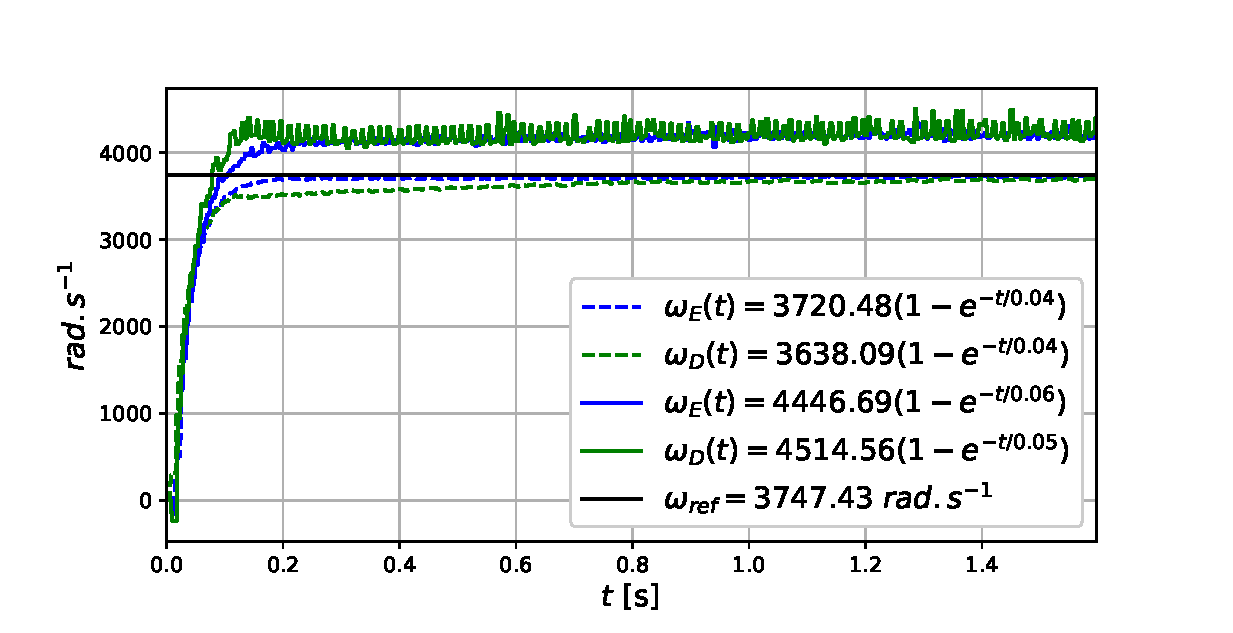
\includegraphics[width=\textwidth]{figuras/resultados/exp02/antes_vs_depois100.eps}
    \caption{Resposta sem observador e sem controle vs com controlador e observador.}
    \end{subfigure}
    
    \caption{Experimento 2. \emph{Sinal de controle e Referência igual a 1.0.}}
    \label{fig:exp02_100}
\end{figure}



\begin{figure}[H]
    % \centering
    \begin{subfigure}{.5\textwidth}
    \centering
    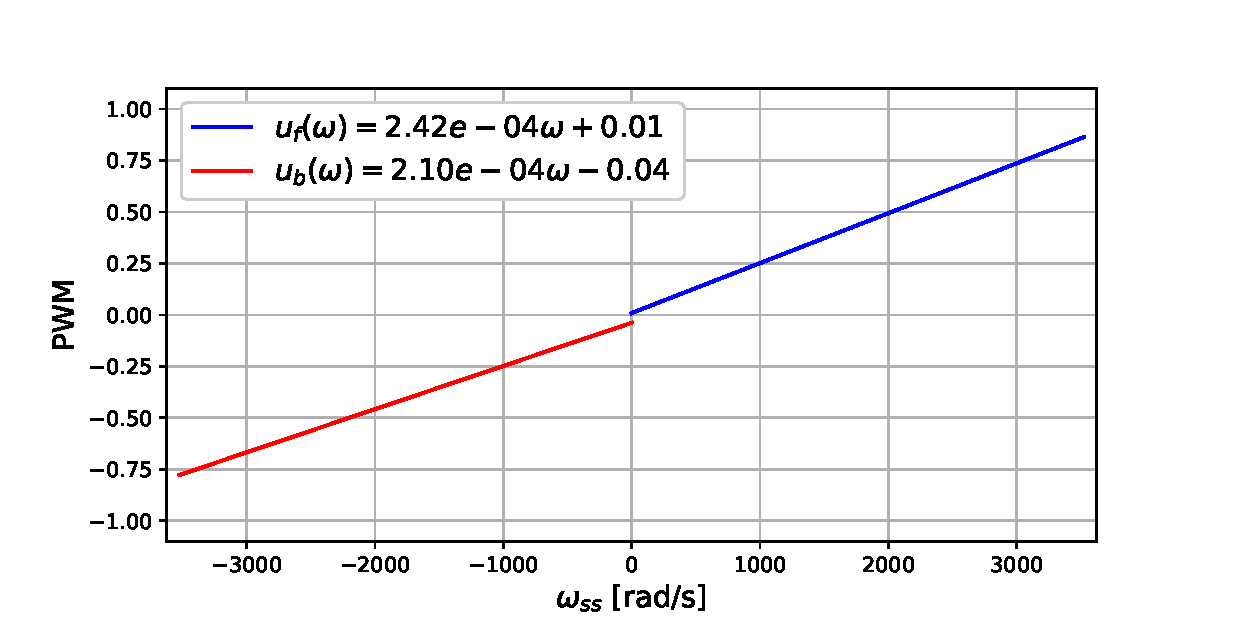
\includegraphics[width=\textwidth]{figuras/resultados/exp03/curva_feedforward_esquerdo100.eps}
    \caption{Curva $u(\omega)$ para o motor esquerdo.}
    \end{subfigure}
    \hfill
    \begin{subfigure}{.5\textwidth}
    \centering
    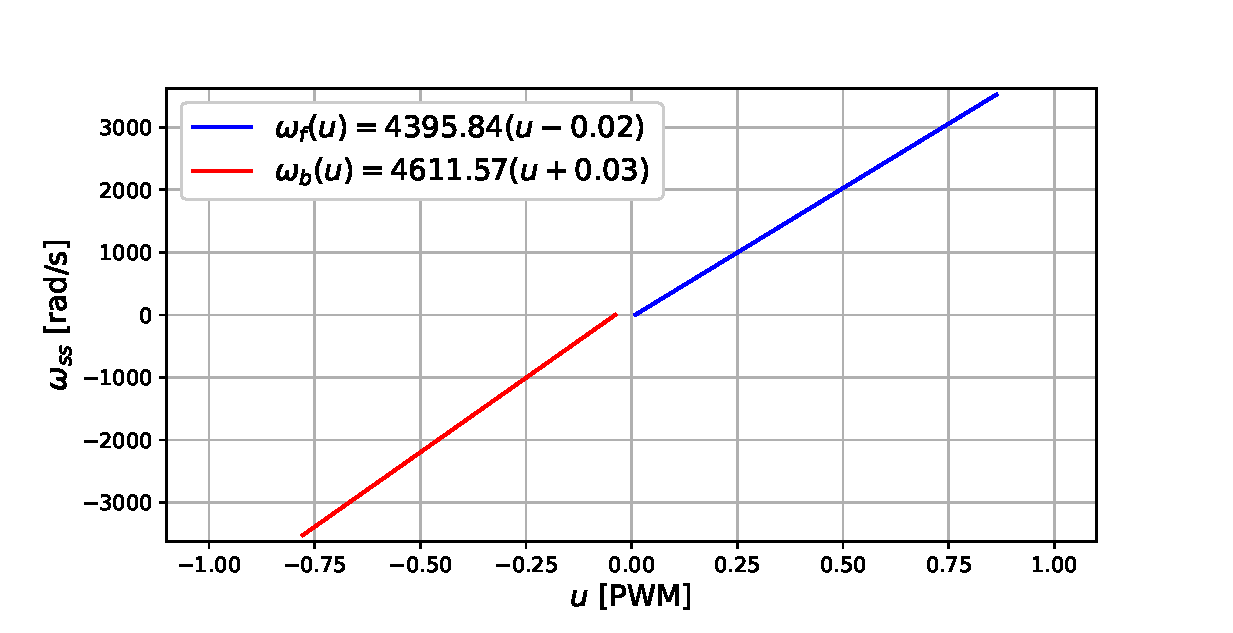
\includegraphics[width=\textwidth]{figuras/resultados/exp03/curva_feedforward_direito100.eps}
    \caption{Curva $u(\omega)$ para o motor direito.}
    \end{subfigure}
    \begin{subfigure}{.5\textwidth}
    \centering
    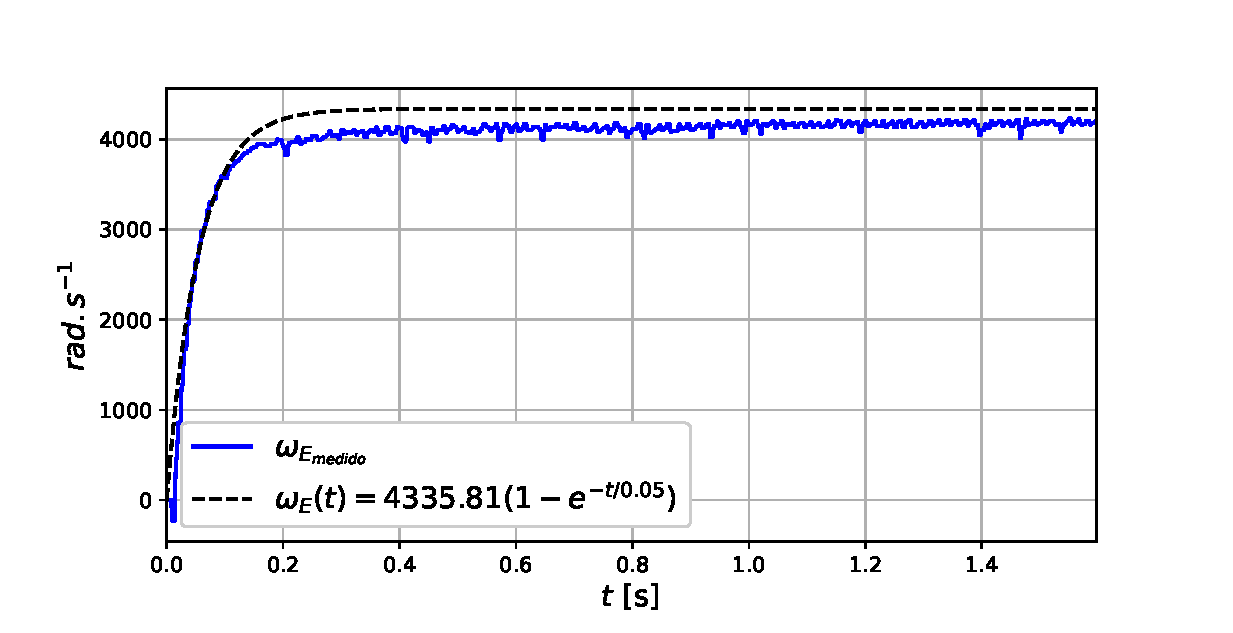
\includegraphics[width=\textwidth]{figuras/resultados/exp03/regressao_vs_medido_esquerdo100.eps}
    \caption{Curva $\omega(t)$ ideal, com os parâmetros da identificação vs velocidades medidas. Motor Esquerdo.}
    \end{subfigure}
    \hfill
    \begin{subfigure}{.5\textwidth}
    \centering
    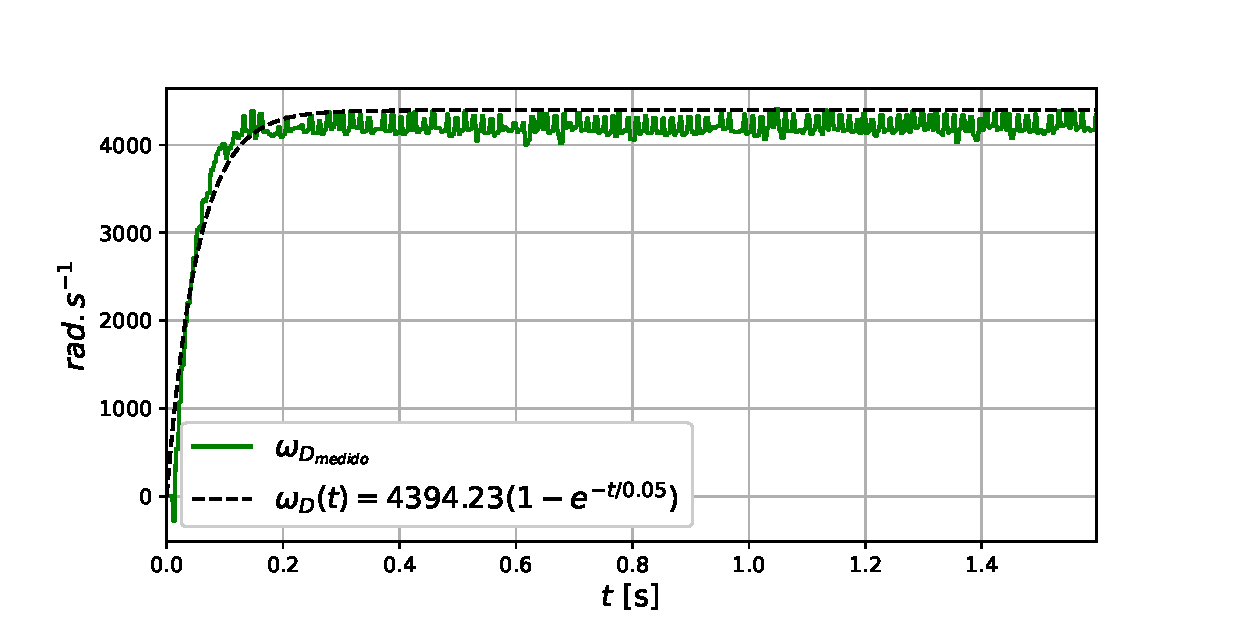
\includegraphics[width=\textwidth]{figuras/resultados/exp03/regressao_vs_medido_direito100.eps}
    \caption{Curva $\omega(t)$ ideal, com os parâmetros da identificação vs velocidades medidas. Motor Direito.}
    \end{subfigure}
    \hfill
    \begin{subfigure}{.5\textwidth}
    \centering
    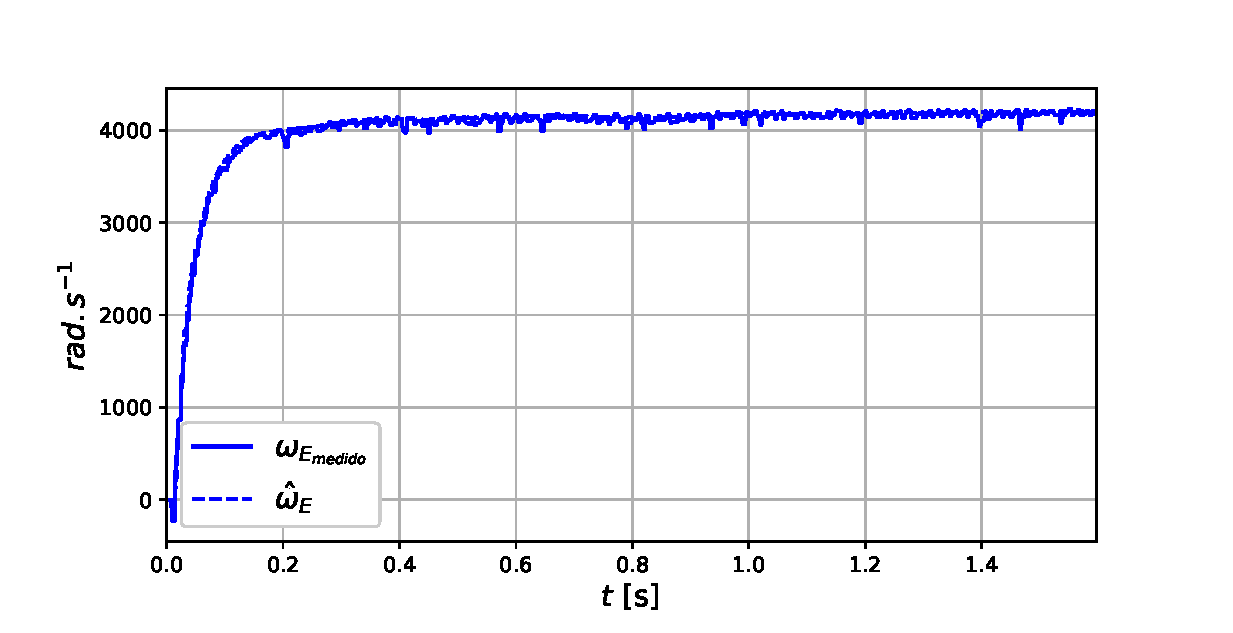
\includegraphics[width=\textwidth]{figuras/resultados/exp03/filtro_vs_sem_filtro_esquerdo100.eps}
    \caption{Comparação entre a velocidade estimativa $\hat{\omega}$ e a velocidade $\omega$ medida. Motor Esquerdo.}
    \end{subfigure}
    \hfill
    \begin{subfigure}{.5\textwidth}
    \centering
    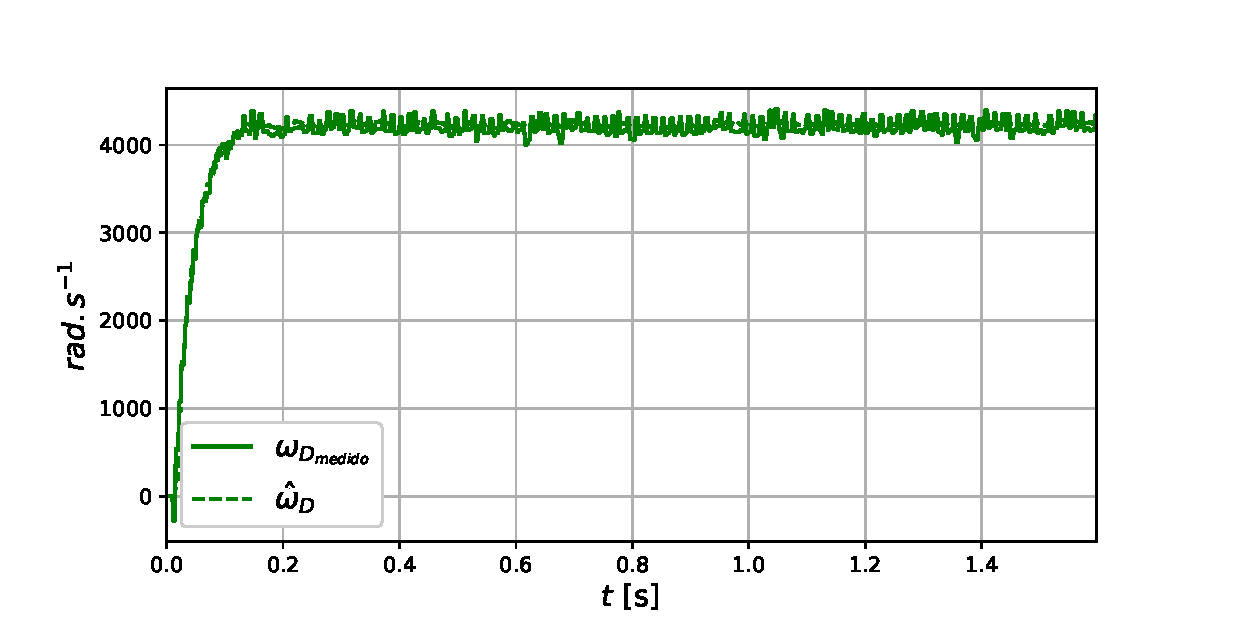
\includegraphics[width=\textwidth]{figuras/resultados/exp03/filtro_vs_sem_filtro_direito100.eps}
    \caption{Comparação entre a velocidade estimativa $\hat{\omega}$ e a velocidade $\omega$ medida. Motor Direito.}
    \end{subfigure}
    \hfill
    \begin{subfigure}{.5\textwidth}
    \centering
    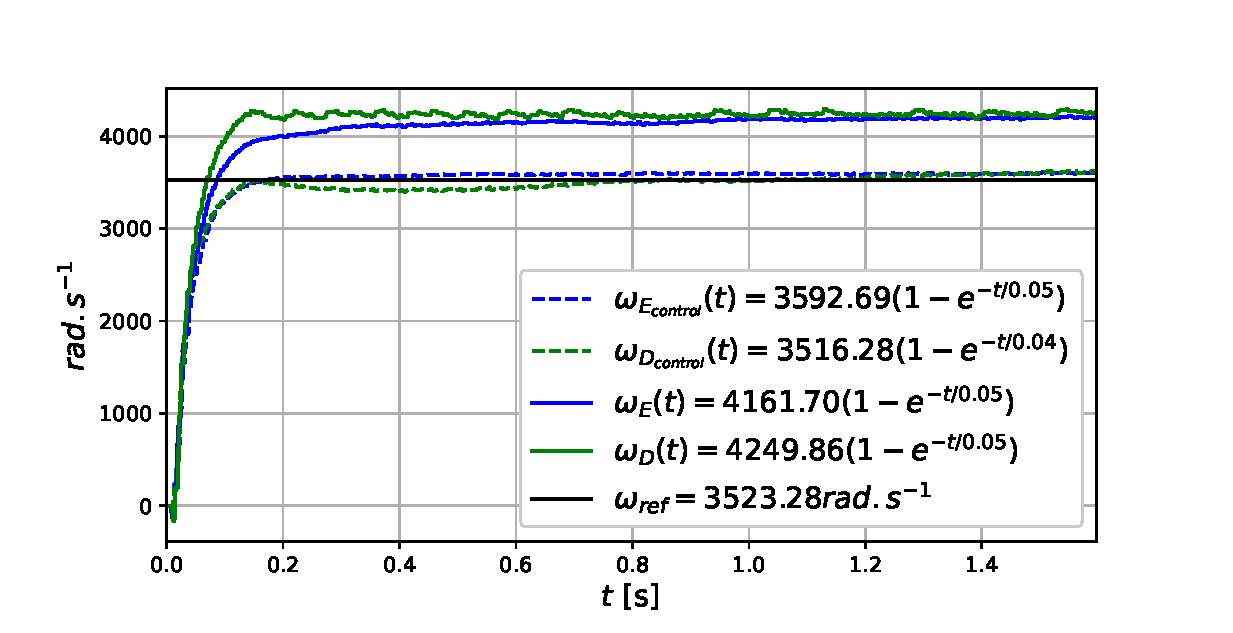
\includegraphics[width=\textwidth]{figuras/resultados/exp03/controlador_vs_sem_controlador100.eps}
    \caption{Comparação entre o sistema com controlador vs sem controlador.}
    \end{subfigure}
    \hfill
    \begin{subfigure}{.5\textwidth}
    \centering
    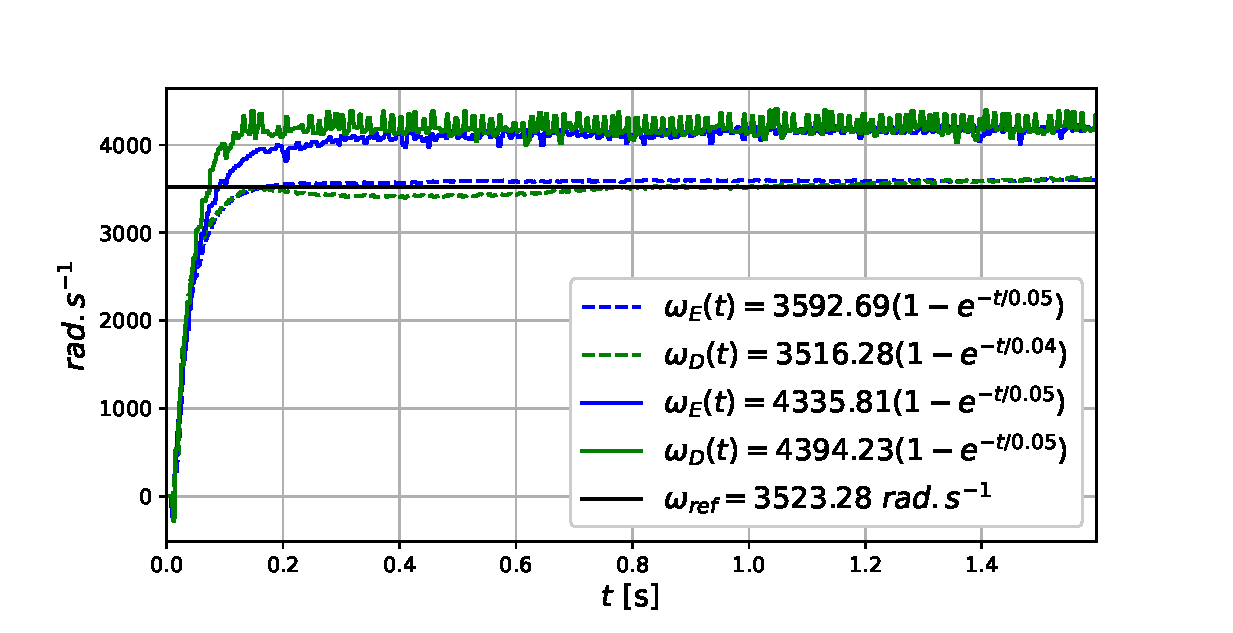
\includegraphics[width=\textwidth]{figuras/resultados/exp03/antes_vs_depois100.eps}
    \caption{Resposta sem observador e sem controle vs com controlador e observador.}
    \end{subfigure}
    
    \caption{Experimento 3. \emph{Sinal de controle e Referência igual a 1.0.}}
    \label{fig:exp03_100}
\end{figure}


\begin{figure}[H]
    % \centering
    \begin{subfigure}{.5\textwidth}
    \centering
    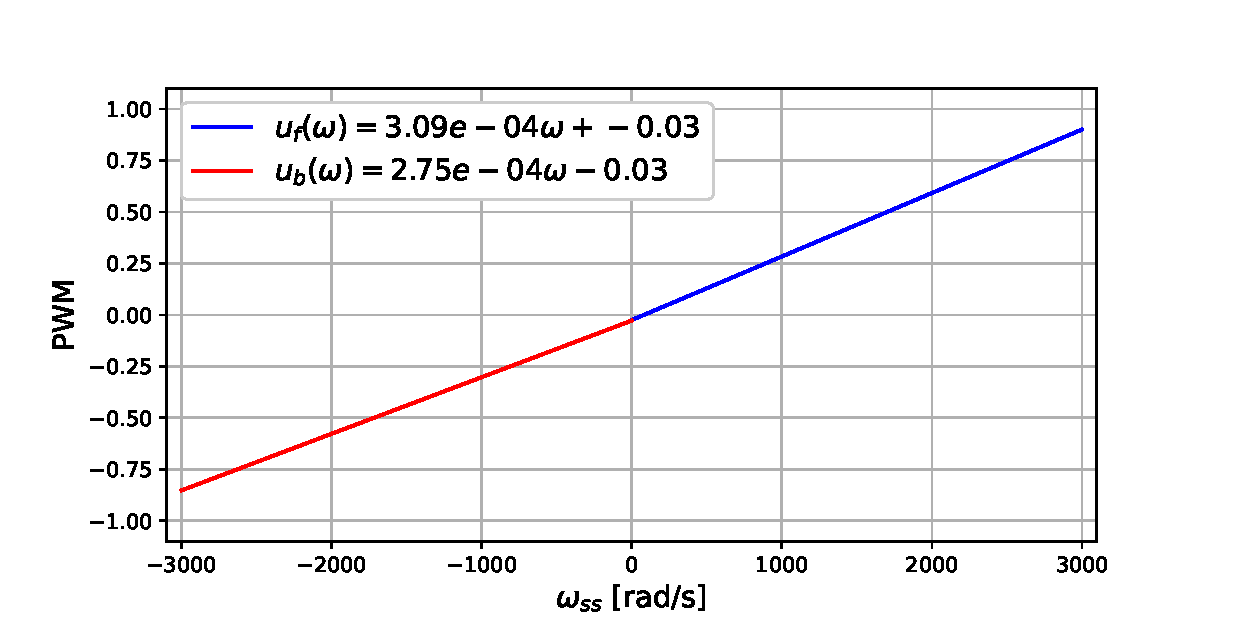
\includegraphics[width=\textwidth]{figuras/resultados/exp04/curva_feedforward_esquerdo100.eps}
    \caption{Curva $u(\omega)$ para o motor esquerdo.}
    \end{subfigure}
    \hfill
    \begin{subfigure}{.5\textwidth}
    \centering
    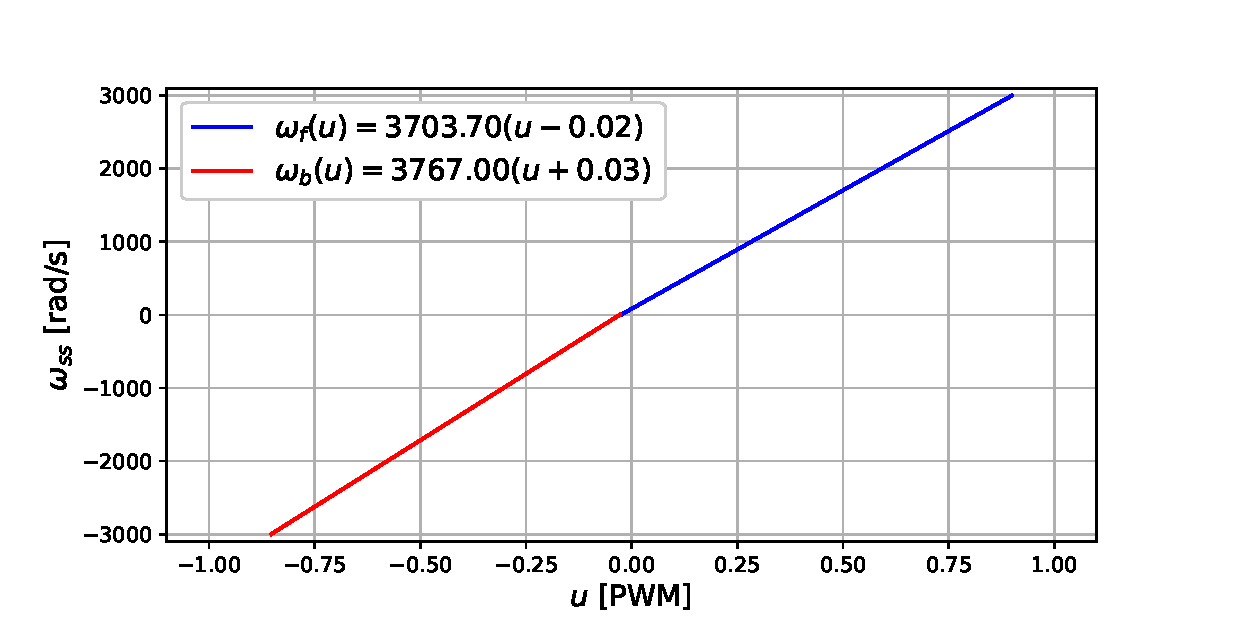
\includegraphics[width=\textwidth]{figuras/resultados/exp04/curva_feedforward_direito100.eps}
    \caption{Curva $u(\omega)$ para o motor direito.}
    \end{subfigure}
    \begin{subfigure}{.5\textwidth}
    \centering
    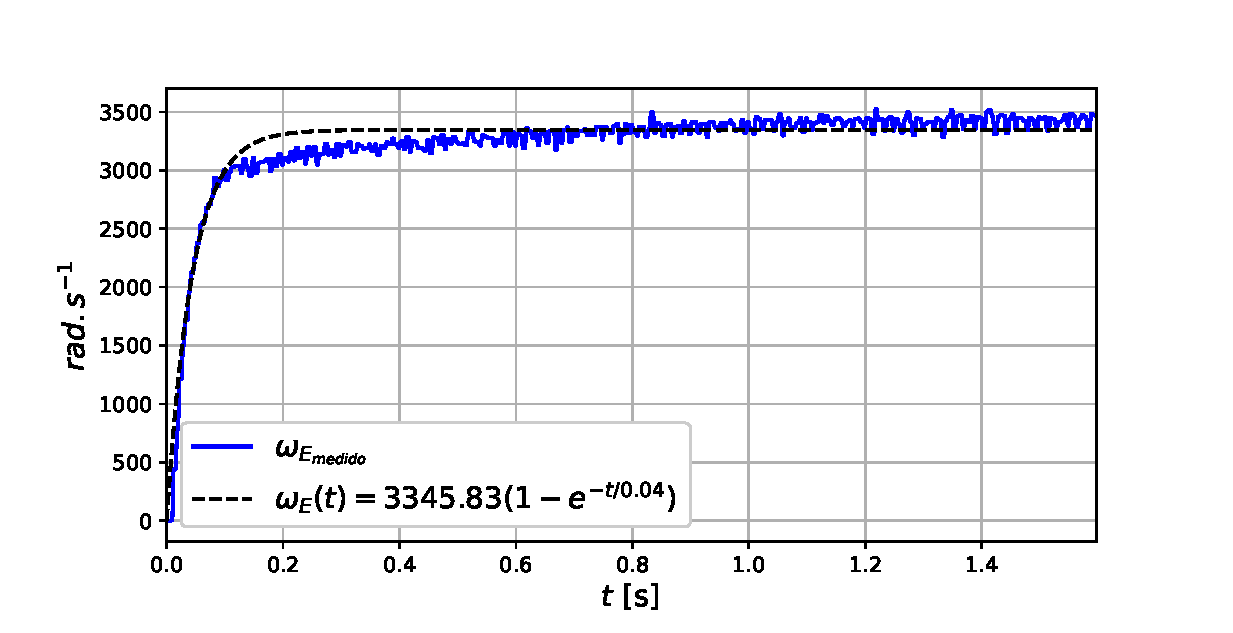
\includegraphics[width=\textwidth]{figuras/resultados/exp04/regressao_vs_medido_esquerdo100.eps}
    \caption{Curva $\omega(t)$ ideal, com os parâmetros da identificação vs velocidades medidas. Motor Esquerdo.}
    \end{subfigure}
    \hfill
    \begin{subfigure}{.5\textwidth}
    \centering
    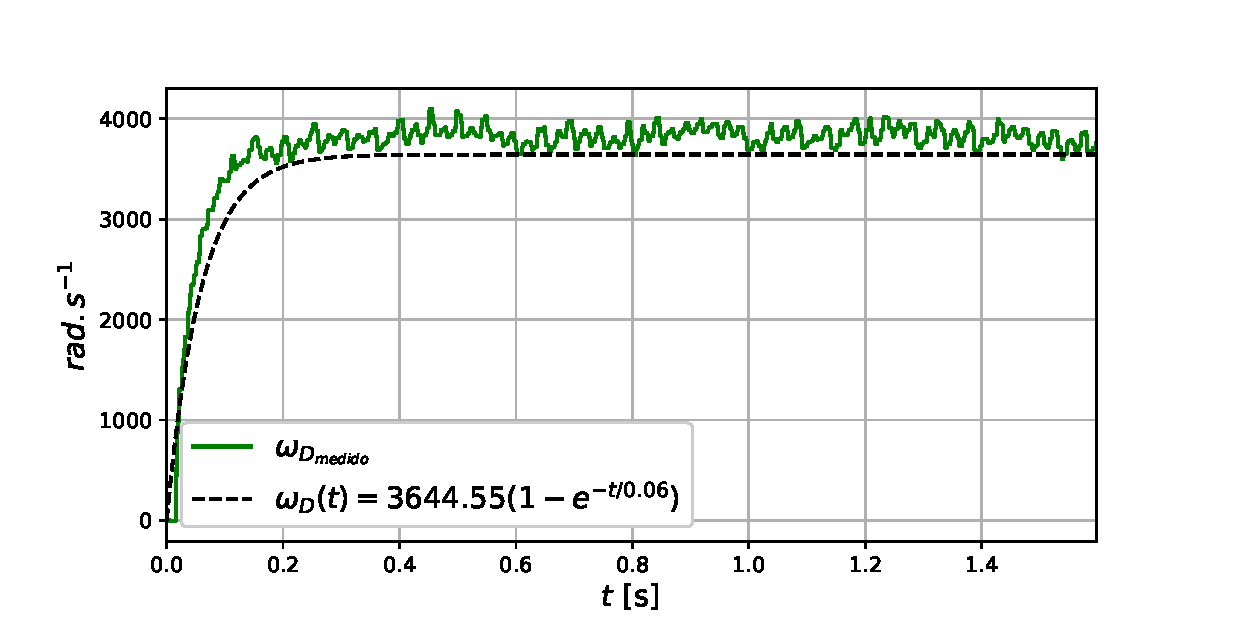
\includegraphics[width=\textwidth]{figuras/resultados/exp04/regressao_vs_medido_direito100.eps}
    \caption{Curva $\omega(t)$ ideal, com os parâmetros da identificação vs velocidades medidas. Motor Direito.}
    \end{subfigure}
    \hfill
    \begin{subfigure}{.5\textwidth}
    \centering
    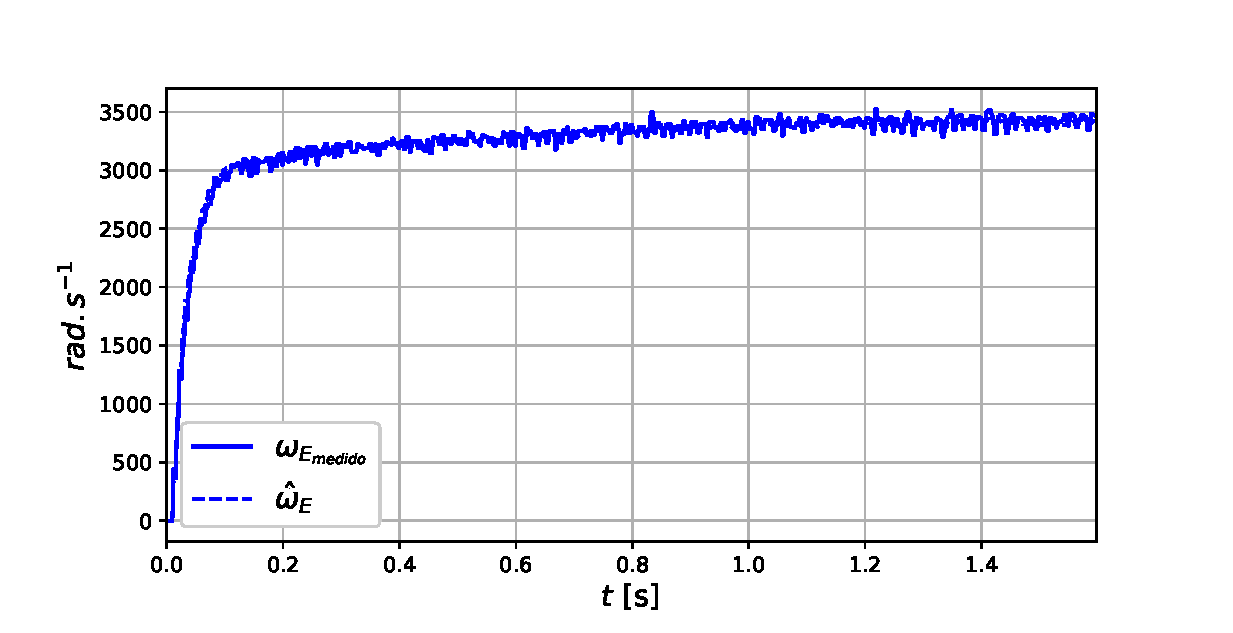
\includegraphics[width=\textwidth]{figuras/resultados/exp04/filtro_vs_sem_filtro_esquerdo100.eps}
    \caption{Comparação entre a velocidade estimativa $\hat{\omega}$ e a velocidade $\omega$ medida. Motor Esquerdo.}
    \end{subfigure}
    \hfill
    \begin{subfigure}{.5\textwidth}
    \centering
    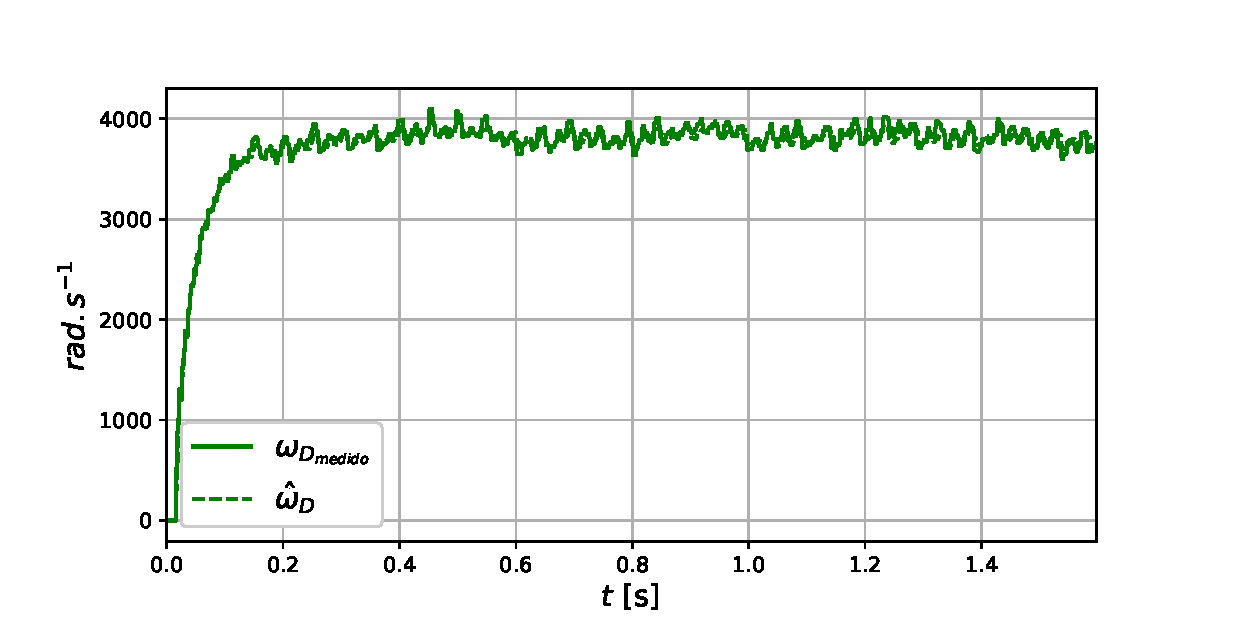
\includegraphics[width=\textwidth]{figuras/resultados/exp04/filtro_vs_sem_filtro_direito100.eps}
    \caption{Comparação entre a velocidade estimativa $\hat{\omega}$ e a velocidade $\omega$ medida. Motor Direito.}
    \end{subfigure}
    \hfill
    \begin{subfigure}{.5\textwidth}
    \centering
    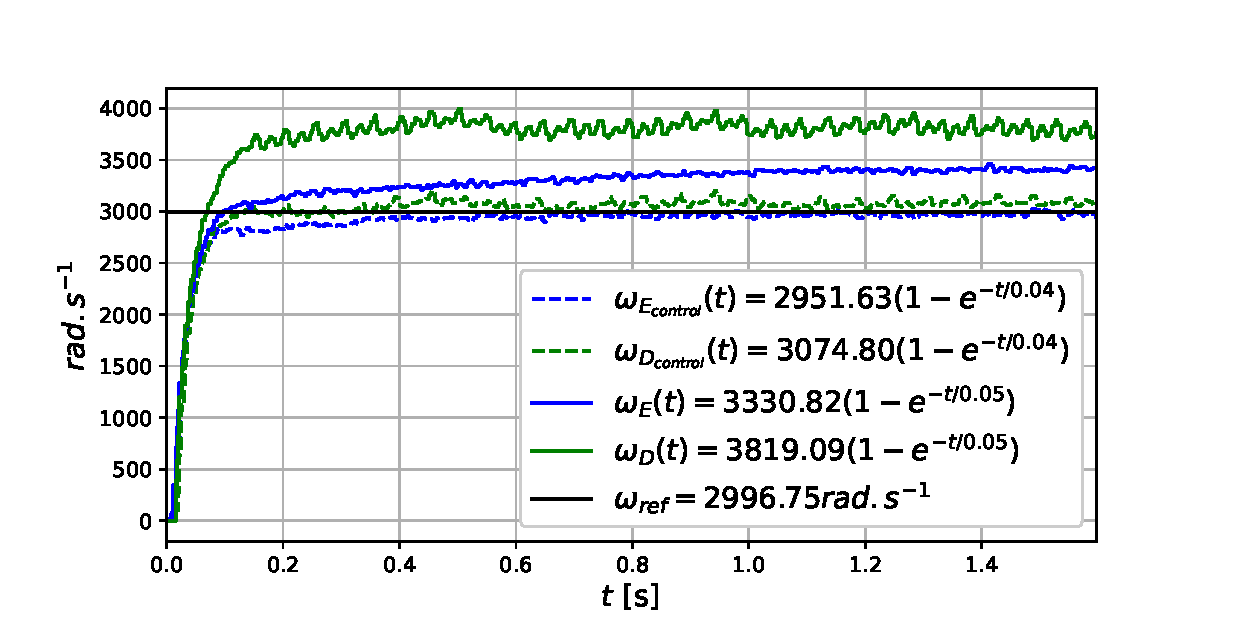
\includegraphics[width=\textwidth]{figuras/resultados/exp04/controlador_vs_sem_controlador100.eps}
    \caption{Comparação entre o sistema com controlador vs sem controlador.}
    \end{subfigure}
    \hfill
    \begin{subfigure}{.5\textwidth}
    \centering
    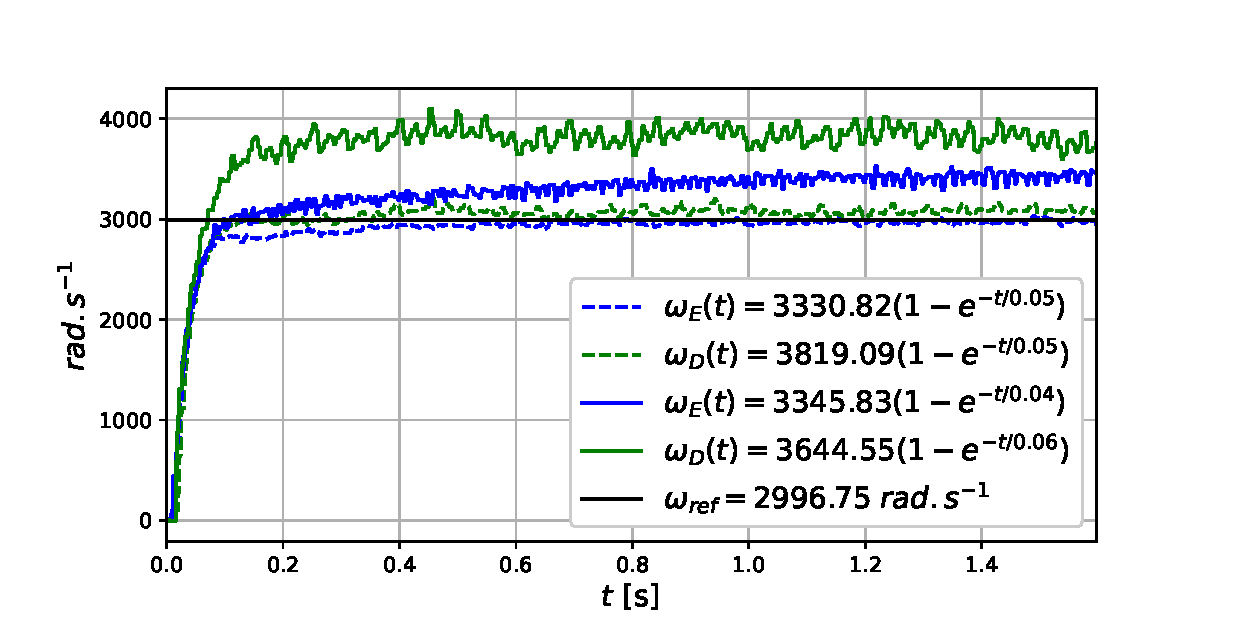
\includegraphics[width=\textwidth]{figuras/resultados/exp04/antes_vs_depois100.eps}
    \caption{Resposta sem observador e sem controle vs com controlador e observador.}
    \end{subfigure}
    
    \caption{Experimento 4. \emph{Sinal de controle e Referência igual a 1.0.}}
    \label{fig:exp04_100}
\end{figure}